%%%%%%%%%%%%%%%%%%%%%%%%%%%%%%%%%%%%%%%%%%%%%%%%%%%%%%%%%%%%%%%%%%%%%
% LaTeX Template: Project Titlepage Modified (v 0.1) by rcx
%
% Original Source: http://www.howtotex.com
% Date: February 2014
% 
% This is a title page template which be used for articles & reports.
% 
% This is the modified version of the original Latex template from
% aforementioned website.
% 
%%%%%%%%%%%%%%%%%%%%%%%%%%%%%%%%%%%%%%%%%%%%%%%%%%%%%%%%%%%%%%%%%%%%%%

\documentclass[12pt]{report}
\usepackage[a4paper]{geometry}
\usepackage[myheadings]{fullpage}
\usepackage{fancyhdr}
\usepackage{lastpage}
\usepackage{graphicx, wrapfig, subcaption, setspace, booktabs}
\usepackage[T1]{fontenc}
\usepackage[font=small, labelfont=bf]{caption}
\usepackage{fourier}
\usepackage[protrusion=true, expansion=true]{microtype}
\usepackage[english]{babel}
\usepackage{sectsty}
\usepackage{url, lipsum}
\usepackage{titlesec}
\usepackage{apacite}

\newcommand{\HRule}[1]{\rule{\linewidth}{#1}}
\onehalfspacing
\setcounter{tocdepth}{5}
\setcounter{secnumdepth}{5}

\titleformat{\chapter}{\normalfont\huge}{\thechapter.}{20pt}{\huge\it}


%-------------------------------------------------------------------------------
% HEADER & FOOTER
%-------------------------------------------------------------------------------
\pagestyle{fancy}
\fancyhf{}
\setlength\headheight{15pt}
\fancyhead[L]{Student ID: 0911576}
\fancyhead[R]{Hogeschool Rotterdam}
\fancyfoot[R]{Page \thepage\ of \pageref{LastPage}}

\fancypagestyle{plain}{%
  \fancyhf{}%
  \setlength\headheight{15pt}
  \fancyhead[L]{Student ID: 0911576}
  \fancyhead[R]{Hogeschool Rotterdam}
  \fancyfoot[R]{Page \thepage\ of \pageref{LastPage}}
}
%-------------------------------------------------------------------------------
% TITLE PAGE
%-------------------------------------------------------------------------------

\begin{document}

\title{ \normalsize \textsc{Rapporteren en Engels}
		\\ [2.0cm]
		\HRule{0.5pt} \\
		\LARGE \textbf{\uppercase{Motion sensors in retirement homes}}
		\HRule{2pt} \\ [0.5cm]
		\normalsize \today \vspace*{5\baselineskip}}

\date{}

\author{
		Mitchell Scheidsbach \\
		Student ID: 0911576 \\ 
		Hogeschool Rotterdam \\
		Technical computer sciences }

\maketitle
\tableofcontents
\newpage

%-------------------------------------------------------------------------------
% Section title formatting
\sectionfont{\scshape}
%-------------------------------------------------------------------------------

%-------------------------------------------------------------------------------
% BODY
%-------------------------------------------------------------------------------
\chapter{Introduction}
\section{Safety issues in retirement homes}
Retirement homes used to be inhabited by elderly that were fairly independent and could help themselves in case of an emergency. Recently the cabinet enacted a policy that made the elderly who can still take care of themselves stay at home longer \cite{Zorgwijzer2017}. As a result of this policy retirement homes are now mostly inhabited by elderly that cannot rescue themselves in case of an emergency. The reason for this are physical limitations or mental problems, such as dementia.

In the year 2015 there were 34 deadly fires resulting in 38 victims. Fifteen percent of those victims lived in a retirement home or a similar health care institution \cite{Kobes2016}. This percentage is so high because of the limited self-reliance of the inhabitants.

On the twelfth of March 2011 a fire arose in the intensive care building in Zorgcentum Rivierduinen in Oegstgeest, the Netherlands \cite{2012}. The patients did not cooperate during the evacuation, which combined with the fire and smoke resulted in confusion about who had and who hadn’t been evacuated from the building. This incident led to three deaths.

My solution to prevent a repeat of this incident is a motion sensor that will be placed in every room of the retirement home which will activate when the fire alarm activates. With this system you will able to easily see where people are still present, and thus increase the chance that the patient can be saved on time.
\begin{figure}[!ht]
	\centering
	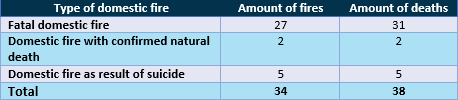
\includegraphics[width=0.6\textwidth]{images/Tabel_Doden_brand.png}
	\caption{Domestic fires resulting in death}
	\centering
	\label{label:file_name}
\end{figure}


\chapter{Elaboration}
\section{My solution is detail}
My solution exists of a network of motion sensors in every room of the retirement home. They will automatically activate when the fire alarm goes off. This way the system will see where there are people present the moment a fire starts, so that they can be easily found and assisted with evacuating the building.

\begin{wrapfigure}{r}{0.30\textwidth}
	\vspace{-40pt}
	\begin{center}
		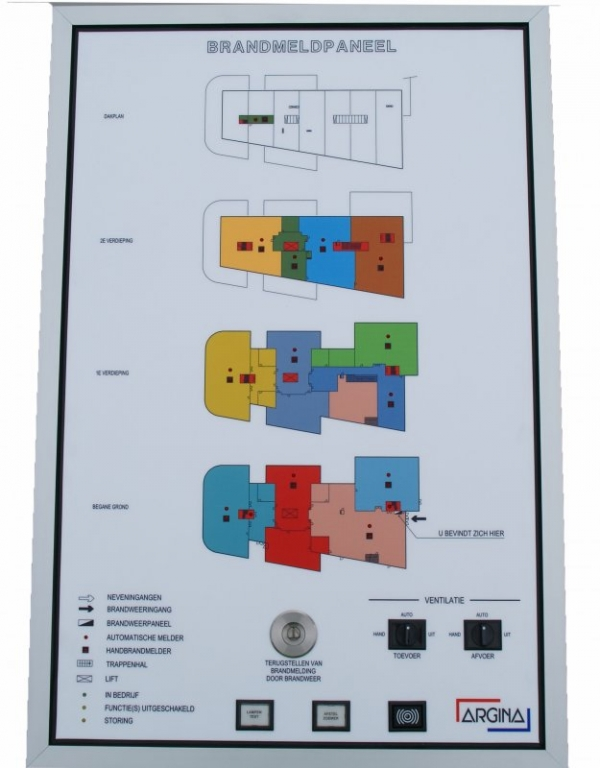
\includegraphics[width=0.35\textwidth]{images/brandpaneel.jpg}
	\end{center}
	\vspace{-20pt}
	\caption{Fire alarm panel}
	\label{label:file_name}
\end{wrapfigure}

Every retirement home has a fire alarm panel \cite{BinnenlandseZakenenKoninkrijksrelaties}. This panel usually consists of a blueprint of the building with red flashing lights on the location of the fire. My solution could make use of this panel by adding differently coloured lights that show where motion has been detected. If this is not a viable possibility then another panel can be made to show the location. It would even be possible to show this information wirelessly so the emergency services can see this information everywhere in the building.

The motion sensors only activate in case of a fire and does not tell who is on the location, only that someone is. This way the system cannot be exploited to track the location of specific patients, so privacy is not compromised.


\section{Why my solution is renewing}
Although retirement homes that use cameras already exist, their implementation works differently than mine \cite{Persoonsgegevens2016}. Usually the cameras get used to see what a patient is doing remotely, which means that a nurse does not have to check up on the patient in person if there are no problems. But when there is a fire the smoke might make it impossible to see anything, rendering them useless when checking a building for people who might be left inside. The motion sensors can be developed in such a way that the smoke becomes a non-issue.


\section{Advantages and Disadvantages}
An advantage of this system is that you can easily see where people are present so that emergency services can immediately go to where they are most needed. The time this will save could be enough to save lives.

A disadvantage is that people might fall unconscious due to the smoke. The motion sensor will not be able to see that someone is present in the room. Checking the rooms for people that need help is still a necessity.

Another advantage is that sensors will still work through smoke. So when there is too much smoke to safely check all the rooms you can check the sensors to see if anyone is present and go straight to them to assist them in evacuating the building.


\chapter{Conclusion}
Basically: my solution to prevent a repeat of the incident at Zorgcentrum Rivierduinen is a network of motion sensors in every room that will automatically activate in case of a fire. The sensors will show the locations where people are still present so that emergency services can quickly rescue people. This will hopefully reduce the amount of fatal victims during a fire.


\bibliographystyle{apacite}
\bibliography{engels_referenties}

\end{document}

%-------------------------------------------------------------------------------
% SNIPPETS
%-------------------------------------------------------------------------------

%\begin{figure}[!ht]
%	\centering
%	\includegraphics[width=0.8\textwidth]{file_name}
%	\caption{}
%	\centering
%	\label{label:file_name}
%\end{figure}

%\begin{figure}[!ht]
%	\centering
%	\includegraphics[width=0.8\textwidth]{graph}
%	\caption{Blood pressure ranges and associated level of hypertension (American Heart Association, 2013).}
%	\centering
%	\label{label:graph}
%\end{figure}

%\begin{wrapfigure}{r}{0.30\textwidth}
%	\vspace{-40pt}
%	\begin{center}
%		\includegraphics[width=0.29\textwidth]{file_name}
%	\end{center}
%	\vspace{-20pt}
%	\caption{}
%	\label{label:file_name}
%\end{wrapfigure}

%\begin{wrapfigure}{r}{0.45\textwidth}
%	\begin{center}
%		\includegraphics[width=0.29\textwidth]{manometer}
%	\end{center}
%	\caption{Aneroid sphygmomanometer with stethoscope (Medicalexpo, 2012).}
%	\label{label:manometer}
%\end{wrapfigure}

%\begin{table}[!ht]\footnotesize
%	\centering
%	\begin{tabular}{cccccc}
%	\toprule
%	\multicolumn{2}{c} {Pearson's correlation test} & \multicolumn{4}{c} {Independent t-test} \\
%	\midrule	
%	\multicolumn{2}{c} {Gender} & \multicolumn{2}{c} {Activity level} & \multicolumn{2}{c} {Gender} \\
%	\midrule
%	Males & Females & 1st level & 6th level & Males & Females \\
%	\midrule
%	\multicolumn{2}{c} {BMI vs. SP} & \multicolumn{2}{c} {Systolic pressure} & \multicolumn{2}{c} {Systolic Pressure} \\
%	\multicolumn{2}{c} {BMI vs. DP} & \multicolumn{2}{c} {Diastolic pressure} & \multicolumn{2}{c} {Diastolic pressure} \\
%	\multicolumn{2}{c} {BMI vs. MAP} & \multicolumn{2}{c} {MAP} & \multicolumn{2}{c} {MAP} \\
%	\multicolumn{2}{c} {W:H ratio vs. SP} & \multicolumn{2}{c} {BMI} & \multicolumn{2}{c} {BMI} \\
%	\multicolumn{2}{c} {W:H ratio vs. DP} & \multicolumn{2}{c} {W:H ratio} & \multicolumn{2}{c} {W:H ratio} \\
%	\multicolumn{2}{c} {W:H ratio vs. MAP} & \multicolumn{2}{c} {\% Body fat} & \multicolumn{2}{c} {\% Body fat} \\
%	\multicolumn{2}{c} {} & \multicolumn{2}{c} {Height} & \multicolumn{2}{c} {Height} \\
%	\multicolumn{2}{c} {} & \multicolumn{2}{c} {Weight} & \multicolumn{2}{c} {Weight} \\
%	\multicolumn{2}{c} {} & \multicolumn{2}{c} {Heart rate} & \multicolumn{2}{c} {Heart rate} \\
%	\bottomrule
%	\end{tabular}
%	\caption{Parameters that were analysed and related statistical test performed for current study. BMI - body mass index; SP - systolic pressure; DP - diastolic pressure; MAP - mean arterial pressure; W:H ratio - waist to hip ratio.}
%	\label{label:tests}
%\end{table}